\subsection{Vectorization}\label{ssec:vectorization}

Vectorization refers to the parallelization of operations on multiple data at the hardware level.
On a modern Intel 64-bit processor supporting AVX, 
four double-precision floating point numbers can be processed simultaneously,
roughly improving performance by a factor of four.
While the compiler optimization is able to vectorize a user's code sometimes, it is not guaranteed
because vectorization requirements are quite stringent. 
For example, vectorization is not guaranteed if memory access is not done in a contiguous fashion
and is impossible if there is any dependency between loop iterations.
This makes it quite challenging to design an AD system that 
can always predict compiler optimization to create vectorized code.
However, vectorization can make AD extremely fast, powerful, and practical even in complex problems.
In practice, we come across many examples where operations can be vectorized during gradient computation.
For example, matrix multiplication, any reduction from a multi-dimensional variable to a scalar such as
summation or product of all elements, and any unary and binary function that is applied element-wise such as
exponential, logarithm, power, sin, cos, tan, and the usual arithmetic operators.

Since most of the opportunities for vectorization occur in matrix operations,
the goal is to use a well-polished and efficient
matrix library such as \code{Eigen}, one of the most popular C++ matrix libraries.
However, this is not an easy task.
Adept2.0 notes in their documentation that integrating an expression-template based matrix library 
such as \code{Eigen} into an AD system can be quite challenging in design.
To circumvent these design issues, 
Adept2.0 integrates their own matrix library designed specifically for their AD system.
This, however, only introduces another problem of writing an efficient matrix library, another daunting task.
In fact, the author of Adept notes that matrix multiplication,
one of the most widely used matrix operations, 
is currently very slow~\cite{hogan:2014}.
Stan mentions that integrating matrix libraries can lead to unexpected problems 
that would require extra memory allocations to resolve~\cite{carpenter:2015}.
Other libraries such as ADOL-C, CppAD, and Sacado do not integrate any matrix libraries directly,
but they do allow the use of \code{Eigen} matrix classes simply as containers.

The one library among those mentioned previously that ultimately incorporates \code{Eigen} is Stan.
Stan provides their own ``plug-ins'', which extend \code{Eigen} classes for their AD variables.
For example, in Stan, one would use \\
\code{Eigen::Matrix<stan::math::var, \ldots>} as a matrix of AD (univariate) variables,
where the generic matrix object is extended to work differently for \code{stan::math::var}.
However, this design still does not take full advantage of the vectorization that \code{Eigen} provides.
One reason is that \code{Eigen} is only highly optimized for matrices of primitive types such as double-precision floating points and integers.
For any other class types, \code{Eigen} defaults to a less optimized version with no guarantees of vectorization.
Therefore, unless one extends all \code{Eigen} methods with optimizations for their specific class type,
they will not receive much benefit of vectorization.
Another reason is that these matrices now have a heterogeneous structure where
each element is an AD variable which represents a pair of value and adjoint.
As a result, it is not possible to read only the values (and similarly, only the adjoints) of the matrix in a contiguous fashion.
The compiler then cannot guarantee any automatic vectorization.

\begin{figure*}[t]
    \centering
    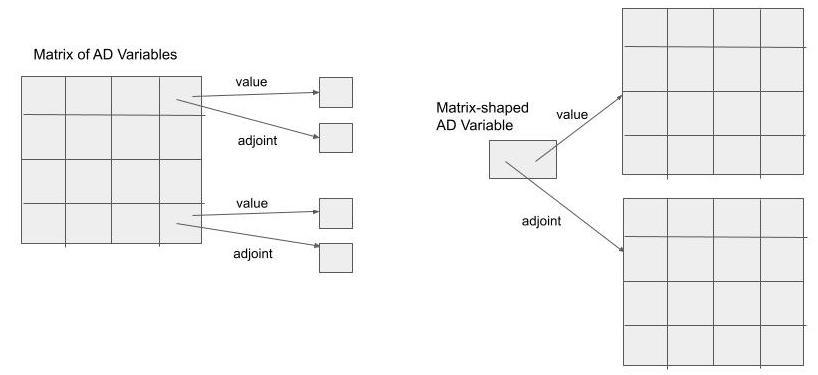
\includegraphics[width=0.8\textwidth]{fastad/figs/matrix-memory-layout.jpg}
    \caption{%
        The left shows the memory layout for a matrix of univariate AD variables.
        This refers to the design pattern ``a matrix of pair of pointers to double''
        since each element of the matrix contains two pointers pointing to its value and adjoint.
        The right shows the memory layout for a single matrix-shaped AD variable,
        referring to the reverse pattern ``a pair of pointers to matrix of doubles''.
        This AD variable has two pointers, each pointing to a matrix of doubles for the value and adjoint.
    }\label{fig:matrix-memory-layout}
\end{figure*}

FastAD fully utilizes the benefits of \code{Eigen} through one simple design difference, which we refer to as \emph{shape traits}.
Stan as well as the other libraries mentioned previously except Adept2.0
follow the design pattern of ``a matrix of pair of pointers to double'' when defining a matrix of AD variables.
Note that a univariate AD variable internally contains two pointers to doubles,
one pointing to the value and one to the adjoint.
In contrast, FastAD follows the reverse pattern: ``a pair of pointers to matrix of doubles''.
That is, rather than defining a univariate AD variable, which gets reused as an element of a matrix,
we define a separate matrix AD variable containing a pair of pointers, each pointing to a matrix of double.
Figure~\ref{fig:matrix-memory-layout} shows the memory layout for each of the design patterns.
This subtle difference provides a few important benefits.
Since the value and adjoint are now represented as matrices of primitive types,
matrix operations will be vectorized.
The second benefit is the significant reduction of memory consumption.
For other libraries, a matrix of AD variables contains two pointers \emph{for each element}.
However, with our design, a single matrix AD variable would only store two pointers
regardless of the size of the matrix.
Hence, if a matrix is $m\times n$, 
the traditional approach has a $O(mn)$ memory consumption for the pointers,
and FastAD approach has a $O(1)$ consumption.

Using templates in C++,
it is easy to unify the API for the different AD variable shapes
by providing an additional template parameter:
\begin{lstlisting}[style=customcpp]
ad::Var<double, ad::scl> x; // scalar shape
ad::Var<double, ad::vec> v; // vector shape
ad::Var<double, ad::mat> m; // matrix shape
\end{lstlisting}

Shape traits also apply for any arbitrary node because
we can deduce the output shape given the input shapes.
The following is a declaration of a generic node representing an
element-wise unary operation, which demonstrates this idea:
\begin{lstlisting}[style=customcpp]
template <class Unary, class ExprType>
struct UnaryNode:
    ValueAdjView<
      typename util::expr_traits<ExprType>::value_t,
      <@\textcolor{red}{typename util::shape\_traits<ExprType>::shape\_t}@>>
{ /*...*/ };
\end{lstlisting}
The portion highlighted in red related to \code{shape\_t}
takes the input expression type \code{ExprType} and deduces its shape type.
Since an element-wise unary operation always has the same shape as its input,
the unary node takes on the same shape.

To verify that FastAD vectorizes more than Stan, 
we performed reverse-AD for a simple summation function $f(x) = \sum\limits_{i=1}^n x_i$
and generated the disassembly for Stan and FastAD~\footnotemark.\@
\footnotetext{github page: https://github.com/JamesYang007/ADBenchmark}
We extracted the part that performs the summation
and compared the instructions to see whether vectorization was taking place.\@
The following is the disassembly for Stan:
\begin{lstlisting}[style=customasm]
L3178:
    movq    (%rax), %rdx
    addq    $8, %rax
    <@\textcolor{red}{vaddsd}@>   8(%rdx), %xmm0, %xmm0 
    cmpq    %rcx, %rax 
    jne L3178
\end{lstlisting}
The instruction used to add is \code{vaddsd},
which is an AVX instruction to add \emph{scalar} double-precision values.
This is not a vectorized instruction, and hence the addition is not done in parallel.
This portion of the disassembly is related to a specialization of an \code{Eigen} class 
responsible for summation with \emph{default traversal},
which is no different from a naive for-loop.

Compare the above disassembly with the one generated for FastAD:
\begin{lstlisting}[style=customasm]
 L3020:
     addq    $8, %rdx
     <@\textcolor{red}{vaddpd}@>  (%rax), %ymm1, %ymm1   
     <@\textcolor{red}{vaddpd}@>  32(%rax), %ymm0, %ymm0 
     addq    $64, %rax
     cmpq    %rdx, %rcx 
     jg  L3020 
\end{lstlisting}
This portion of the assembly is indeed related to the \emph{linear vectorized traversal}
specialization of the same \code{Eigen} class responsible for the summation.
The instruction used to add is \code{vaddpd},
which is an AVX instruction to add \emph{packed} double-precision values.
This is a vectorized instruction and the operation is truly done in parallel.

Sometimes, Stan is able to produce vectorized code such as in matrix multiplication.
This is consistent with our benchmark results 
since Stan came closest to FastAD for this operation (see Section~\ref{ssec:matrix_mult}).
It is also consistent with how it is implemented,
since they allocate extra memory for \code{double} values for each matrix 
and the multiplication is carried out with these matrices of primitive types.
However, this vectorization does come at a cost of at least 4 times extra memory allocation than what FastAD allocates.
Moreover, the backward-evaluation requires heap-allocating a matrix on-the-fly every time.
FastAD incurs no such cost, only allocates what is needed, and never heap-allocates during AD evaluation.
